\documentclass[twoside,11pt]{article}

\usepackage{jrnl}

\usepackage{geometry}

\usepackage[utf8]{inputenc}
\usepackage[T1]{fontenc}
\usepackage{url}
\usepackage{nicefrac}
\usepackage{microtype}

\usepackage{graphicx}
\usepackage[font=small,labelfont=bf]{caption}
\usepackage{subcaption}
\usepackage{adjustbox}
\usepackage{wrapfig}
\graphicspath{{figures/pdf/}}
\DeclareGraphicsExtensions{.pdf}

\usepackage{tikz}
\usetikzlibrary{bayesnet}
\usetikzlibrary{calc}
\usetikzlibrary{shapes}

\usepackage{comment}

\usepackage{amsfonts}
\usepackage{amsmath}
\usepackage{amssymb}
\usepackage{mathtools}

\usepackage{algorithm}
\usepackage{algorithmic}
\usepackage{rotating}

\usepackage{booktabs}
\usepackage{makecell}
\usepackage{multirow}
\usepackage{tabularx}

\usepackage{enumitem}
\usepackage{xspace}

\usepackage{macro}

\jmlrheading{}{}{}{}{}{}{}
\ShortHeadings{Contextual Explanation Networks}{Al-Shedivat, Dubey, Xing}
\firstpageno{1}

\begin{document}

\title{Contextual Explanation Networks}

\author{\name{Maruan~Al-Shedivat} \email{alshedivat@cs.cmu.edu} \\
  \addr{Carnegie Mellon University}
  \AND
  \name{Avinava~Dubey} \email{avinava.dubey@google.com} \\
  \addr{Google Research}
  \AND
  \name{Eric~P.~Xing} \email{epxing@cs.cmu.edu} \\
  \addr{Carnegie Mellon University \& Petuum Inc.}}

\editor{Edoardo M. Airoldi}

\maketitle


\begin{abstract}Modern learning algorithms excel at producing accurate but complex models of the data.
However, deploying such models in the real-world requires extra care: we must ensure their reliability, robustness, and absence of undesired biases.
This motivates the development of models that are equally accurate but can be also easily inspected and assessed beyond their predictive performance.
To this end, we introduce \emph{contextual explanation networks} ({\CENs})---a class of architectures that learn to predict by generating and utilizing intermediate, simplified probabilistic models.
Specifically, {\CENs} generate parameters for intermediate graphical models which are further used for prediction and play the role of explanations.
Contrary to the existing \emph{post-hoc} model-explanation tools, {\CENs} learn to predict and to explain simultaneously.
Our approach offers two major advantages: (i) for each prediction, valid, instance-specific explanation is generated with no computational overhead and (ii) prediction via explanation acts as a regularizer and boosts performance in data-scarce settings.
We analyze the proposed framework theoretically and experimentally.
Our results on image and text classification and survival analysis tasks demonstrate that {\CENs} are not only competitive with the state-of-the-art methods but also offer additional insights behind each prediction, that can be valuable for decision support.
We also show that while post-hoc methods may produce misleading explanations in certain cases, {\CENs} are consistent and allow to detect such cases systematically.
\end{abstract}
 
\section{Introduction}\label{sec:introduction}

Model interpretability is a long-standing problem in machine learning that has become quite acute with the accelerating pace of the widespread adoption of complex predictive algorithms.
While high performance often supports our belief in the predictive capabilities of a system, perturbation analysis reveals that black-box models can be easily broken in an unintuitive and unexpected manner \citep{szegedy2013intriguing,nguyen2015deep}.
Therefore, for a machine learning system to be used in a social context (\eg, in healthcare) it is imperative to provide sound reasoning for each prediction or decision it makes.

To design such systems, we may restrict the class of models to only \emph{human-intelligible} \citep{caruana2015intelligible}.
However, such an approach is often limiting in modern practical settings.
Alternatively, we may fit a complex model and explain its predictions \emph{post-hoc}, \eg, by searching for linear local approximations of the decision boundary~\citep{ribeiro2016trust}.
While such methods achieve their goal, explanations are generated \emph{a posteriori} require additional computation per data instance and, most importantly, are never the basis for the predictions made in the first place, which may lead to erroneous interpretations, as we show in this paper, or even be exploited~\citep{dombrowski2019explanations, lakkaraju2019fool}.


\begin{figure}[t]
    \centering
    \includegraphics[width=0.60\textwidth]{cen-illustration}\caption{High-level functionality of {\CENs}:
        The context is represented by satellite imagery and used to generate instance-specific linear models (explanations).
        The latter act on a set of interpretable attributes from regional survey data and produce predictions.}
    \label{fig:illustration}
\end{figure}
 
Explanation is a fundamental part of the human learning and decision process~\citep{lombrozo2006structure}.
Inspired by this fact, we introduce \emph{contextual explanation networks} ({\CENs})---a class of architectures that learn to predict and to explain jointly, alleviating the drawbacks of the post-hoc methods.
To make a prediction, {\CENs} operate as follows (Figure~\ref{fig:illustration}).
First, they process a subset of inputs and generate parameters for a simple probabilistic model (\eg, sparse linear model) which is regarded interpretable by a domain expert.
Then, the generated model is applied to another subset of inputs and produces a prediction.
To motivate such an architecture, we consider the following example.

\paragraph{A motivating illustration.}
One of the tasks we consider in this paper is classification of households into poor and not poor having access to satellite imagery and categorical data from surveys~\citep{jean2016combining}.
If a human were to solve this task, to make predictions, they might assign weights to features in the categorical data and explain their predictions in terms of the most relevant variables (\ie, come up with a linear model).
Moreover, depending on the type of the area (as seen from the imagery), they might select slightly different weights for different areas (\emph{e.g.}, when features indicative of poverty are different for urban, rural, and other types of areas).

The {\CEN} architecture given in Figure~\ref{fig:illustration} imitates this process by making predictions using sparse linear models applied to interpretable categorical features.
The weights of the linear models are contextual, generated by a learned encoder that maps images (the context) to the weight vectors.
The learned encoder is sensitive to the infrastructure presented in the input images and generates different linear models for urban and rural areas.
The generated models not only are used for prediction but also play the role of explanations and can encode arbitrary prior knowledge.
{\CENs} can represent complex model classes by using powerful encoders.
At the same time, by offsetting complexity into the encoding process, we achieve simplicity of explanations and can interpret predictions in terms the variables of interest.

The proposed architecture opens a number of questions:
What are the fundamental advantages and limitations of {\CEN}?
How much of the performance should be attributed to the context encoder and how much to the explanations?
Are there any degenerate cases and do they happen in practice?
Finally, how do \CEN-generated explanations compare to alternatives, \eg, produced with \LIME~\citep{ribeiro2016trust}?
In the rest of this paper, we formalize our intuitions and answer these questions theoretically and experimentally.

\subsection{Contributions}\label{sec:contributions}

The main four contributions of this paper are as follows:
\begin{itemize}[noitemsep,topsep=6pt,parsep=2pt,leftmargin=2em]
    \item[(i)] We formally define {\CENs} as a class of probabilistic models, consider special cases, and derive learning and inference algorithms for scalar and structured outputs.

    \item[(ii)] We design {\CENs} in the form of new deep learning architectures trainable end-to-end for prediction and survival analysis tasks.

    \item[(iii)] Empirically, we demonstrate the value of learning with explanations for both prediction and model diagnostics.
    Moreover, we find that explanations can act as a regularizer and result in improved sample efficiency.

    \item[(iv)] We also show that noisy features can render post-hoc explanations inconsistent and misleading, and how {\CENs} can help to detect and avoid such situations.

\end{itemize}

\noindent Our code is available at \url{https://github.com/alshedivat/cen}.

\subsection{Organization}
\label{sec:organization}

The paper is organized as follows.
Section~\ref{sec:background} presents the notation and some background on post-hoc interpretability methods.
In Sections \ref{sec:CEN}, we introduce the general {\CEN} framework, describe specific implementations, learning, and inference.
In Section~\ref{sec:related_work}, we overview broadly related work.
In Section~\ref{sec:analysis}, we discuss and analyze properties of {\CEN} theoretically.
Section~\ref{sec:case-studies} presents a number of case studies:
experimental results for scalar prediction tasks (Section~\ref{sec:applications-classification}),
an empirical analysis of consistency of linear explanations generated by {\CEN} vs. alternatives (Section~\ref{sec:applications-properties}),
and finally how {\CENs} with structured explanations can efficiently solve survival analysis tasks (Section~\ref{sec:applications-survival-analysis}).
 
\section{Background}
\label{sec:background}

We start by introducing the notation and reviewing post-hoc model explanations, with a focus on {\LIME}~\citep{ribeiro2016trust} as one of the most popular frameworks to date.

Given a collection of data where each instance is represented by inputs, , and targets, , our goal is to learn an accurate predictive model, .
To explain predictions, we can assume that each data point has another set of features, .
We construct explanations in the form of simpler models, , so that they are consistent with the original model in the neighborhood of the corresponding data instance, \ie, .
While the original inputs, , can be of complex, low-level, unstructured data types (\eg, text, image pixels, sensory inputs), we assume that  are high-level, meaningful variables (\eg, categorical features).
In the post-hoc explanation literature, it is assumed that  are \emph{derived} from  and are often binary~\citep{lundberg2017shap} (\eg,  can be images, while  can be vectors of binary indicators over the corresponding super-pixels).
We consider a more general setting where  and  are not necessarily derived from each other.
Throughout the paper, we call  the \emph{context} and  the \emph{attributes} or \emph{variables of interest}.

\subsection*{Locally Interpretable Model-agnostic Explanations (LIME)}
\label{sec:lime}

Given a trained model, , and a data instance with features , LIME constructs an explanation, , as follows:

where  is the loss that measures how well  approximates  in the neighborhood defined by the similarity kernel, , in the space of attributes, , and  is the penalty on the complexity of explanation.\footnote{\citet{ribeiro2016trust} argue that only simple models of low complexity (\eg, sufficiently sparse linear models) are human-interpretable and support that by human studies.}
Now more specifically, \citet{ribeiro2016trust} assume that  is the class of linear models, , and define the loss and the similarity kernel as follows:

where the data instance of interest is represented by ,  and the corresponding  are the perturbed features,  is some distance function, and  is the scale parameter of the kernel.
The regularizer, , is often chosen to favor sparse explanations.

The model-agnostic property is the key advantage of LIME (and variations)---we can solve \eqref{eq:LIME-general} for any trained model, , any class of explanations, , at any point of interest, .
While elegant, predictive and explanatory models in this framework are learned independently and hence never affect each other.
In the next section, we propose a class of models that ties prediction and explanation together in a joint probabilistic framework.
 
\section{Contextual Explanation Networks}
\label{sec:CEN}


\begin{figure}[t]
\centering
\begin{subfigure}[b]{0.16\textwidth}
    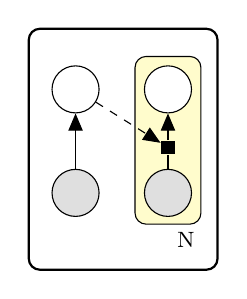
\begin{tikzpicture}[
        inner/.style={draw, fill=yellow!20, thin, inner sep=2pt},
    ]
        \tikzstyle{latent} = [circle,fill=white,draw=black,inner sep=1pt,
        minimum size=17pt, font=\fontsize{9}{9}\selectfont, node distance=1]

        \node (C) [obs] {};
        \node (theta) [latent, above=20pt of C] {};
        \node (X_) [obs, transparent, right=15pt of C, yshift=6pt] {};
        \node (Y_) [obs, transparent, above=15pt of X_, xshift=2pt] {};
        \node (theta_)  [latent, transparent, above=25pt of C] {};

        \node (w) [const, above=5pt of C, xshift=-7pt] {};

        \plate[inner sep=8pt, thick] {CEN} {(C)(theta_)(Y_)} {N};
        \plate[inner] {CRF} {(X_)(Y_)} { };

        \node (X1) [obs, right=16pt of C]  {};
        \node (Y1) [latent, above=20pt of X1] {};

        \edge {C} {theta};

        \factor[above=5pt of X1]{X1-Y1} {} {} {};
        \factoredge {X1} {X1-Y1} {Y1};
        \edge[bend right=25, dashed] {theta} {X1-Y1};
    \end{tikzpicture}
    \caption{}\label{fig:CEN-scalar}
\end{subfigure}
\hfil
\begin{subfigure}[b]{0.29\textwidth}
    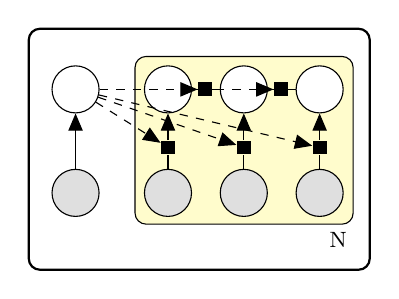
\begin{tikzpicture}[
        inner/.style={draw, fill=yellow!20, thin, inner sep=2pt},
    ]
        \tikzstyle{latent} = [circle,fill=white,draw=black,inner sep=1pt,
        minimum size=17pt, font=\fontsize{9}{9}\selectfont, node distance=1]

        \node (C) [obs] {};
        \node (theta) [latent, above=20pt of C] {};
        \node (X_) [obs, transparent, right=15pt of C, yshift=6pt] {};
        \node (Y_) [obs, transparent, above=15pt of X_, xshift=57pt] {};
        \node (theta_)  [latent, transparent, above=25pt of C] {};

        \node (w) [const, above=5pt of C, xshift=-7pt] {};

        \plate[inner sep=8pt, thick] {CEN} {(C)(theta_)(Y_)} {N};
        \plate[inner] {CRF} {(X_)(Y_)} { };

        \node (X1) [obs, right=16pt of C]  {};
        \node (Y1) [latent, above=20pt of X1] {};
        \node (X2) [obs, right=10pt of X1] {};
        \node (Y2) [latent, right=10pt of Y1] {};
        \node (X3) [obs, right=10pt of X2] {};
        \node (Y3) [latent, right=10pt of Y2] {};

        \edge {C} {theta};

        \factor[above=5pt of X1]{X1-Y1} {} {} {};
        \factoredge {X1} {X1-Y1} {Y1};
        \edge[bend right=25, dashed] {theta} {X1-Y1};

        \factor[above=5pt of X2]{X2-Y2} {} {} {};
        \factoredge {X2} {X2-Y2} {Y2};
        \edge[bend right=18, dashed] {theta} {X2-Y2};

        \factor[above=5pt of X3]{X3-Y3} {} {} {};
        \factoredge {X3} {X3-Y3} {Y3};
        \edge[bend right=12, dashed] {theta} {X3-Y3};

        \factor[right=2pt of Y1]{Y1-Y2} {} {} {};
        \factor[right=2pt of Y2]{Y2-Y3} {} {} {};
        \edge[-] {Y1} {Y2};
        \edge[-] {Y2} {Y3};
        \edge[bend left=50, dashed] {theta} {Y1-Y2};
        \edge[bend left=50, dashed] {theta} {Y2-Y3};
    \end{tikzpicture}
    \caption{}\label{fig:CEN-structured}
\end{subfigure}
\hfil
\begin{subfigure}[b]{0.29\textwidth}
    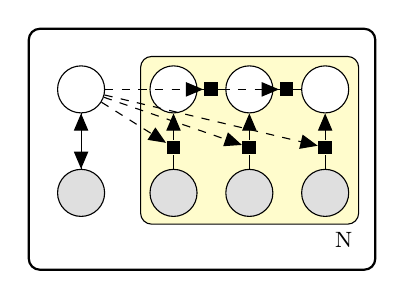
\begin{tikzpicture}[
        inner/.style={draw, fill=yellow!20, thin, inner sep=2pt},
    ]
        \tikzstyle{latent} = [circle,fill=white,draw=black,inner sep=1pt,
        minimum size=17pt, font=\fontsize{9}{9}\selectfont, node distance=1]

        \node (C) [obs] {};
        \node (theta) [latent, above=20pt of C] {};
        \node (C_) [obs, transparent, xshift=-2pt] {};
        \node (X_) [obs, transparent, right=15pt of C, yshift=6pt] {};
        \node (Y_) [obs, transparent, above=15pt of X_, xshift=57pt] {};
        \node (theta_)  [latent, transparent, above=25pt of C] {};

        \node (p) [const, above=8pt of C, xshift=5pt] {};
        \node (q) [const, above=8pt of C, xshift=-13pt] {};

        \plate[inner sep=8pt, thick] {CEN} {(C_)(theta_)(Y_)} {N};
        \plate[inner] {CRF} {(X_)(Y_)} { };

        \node (X1) [obs, right=16pt of C]  {};
        \node (Y1) [latent, above=20pt of X1] {};
        \node (X2) [obs, right=10pt of X1] {};
        \node (Y2) [latent, right=10pt of Y1] {};
        \node (X3) [obs, right=10pt of X2] {};
        \node (Y3) [latent, right=10pt of Y2] {};

        \edge {theta} {C};
        \edge[bend left=30, dashed] {C} {theta};

        \factor[above=5pt of X1]{X1-Y1} {} {} {};
        \factoredge {X1} {X1-Y1} {Y1};
        \edge[bend right=25, dashed] {theta} {X1-Y1};

        \factor[above=5pt of X2]{X2-Y2} {} {} {};
        \factoredge {X2} {X2-Y2} {Y2};
        \edge[bend right=18, dashed] {theta} {X2-Y2};

        \factor[above=5pt of X3]{X3-Y3} {} {} {};
        \factoredge {X3} {X3-Y3} {Y3};
        \edge[bend right=12, dashed] {theta} {X3-Y3};

        \factor[right=2pt of Y1]{Y1-Y2} {} {} {};
        \factor[right=2pt of Y2]{Y2-Y3} {} {} {};
        \edge[-] {Y1} {Y2};
        \edge[-] {Y2} {Y3};
        \edge[bend left=50, dashed] {theta} {Y1-Y2};
        \edge[bend left=50, dashed] {theta} {Y2-Y3};
    \end{tikzpicture}
    \caption{}\label{fig:VCEN}
\end{subfigure}\caption{(a) A graphical model for {\CEN} with a context encoder parameterized by  and linear explanations.
(b) A graphical model for {\CEN} with context encoder and CRF-based explanations.
The model is parameterized by .
(c) A graphical model for {\CEN} with context autoencoding via the inference, , and generator, , networks and CRF-based explanations.}
\label{fig:PGM}
\end{figure}
 
We consider the same problem of learning from a collection of data represented by context variables, , attributes, , and targets, .
We denote the corresponding random variables by capital letters, , , and , respectively.
Our goal is to learn a model, , parametrized by  that can predict  from  and .
We define contextual explanation networks as probabilistic models that assume the following form (Figure~\ref{fig:PGM}):\footnote{While we focus on predictive modeling, {\CENs} are applicable beyond that.
For example, instead of learning a predictive distribution, , we may want to learn a contextual marginal distribution, , over a set random variables , where  is defined by an arbitrary graphical model.}

where  is a predictor parametrized by .
We call such predictors \emph{explanations}, since they explicitly relate interpretable attributes, , to the targets, .
For example, when the targets are scalar and binary, explanations may take the form of linear logistic models;
when the targets are more complex, dependencies between the components of  can be represented by a graphical model, \eg, \emph{conditional random field}~\citep{lafferty2001crf}.

{\CENs} assume that each explanation is context-specific:  defines a conditional probability of an explanation  being valid in the context .
To make a prediction, we marginalize out .
To interpret a prediction, , for a given data instance, , we infer the posterior, .
The main advantage of this approach is to allow modeling conditional probabilities, , in a black-box fashion while keeping the class of explanations, , simple and interpretable.
For instance, when the context is given as raw text, we may choose  to be represented with a recurrent neural network, while  be in the class of linear models.

Implications of these assumptions are discussed in Section~\ref{sec:analysis}.
Here, we continue with a discussion of a number of practical choices for  and  (Table~\ref{tab:cen-components}).


\begin{table}[t!]
\caption{\small Different types of encoders and explanations used in {\CEN}.}
\label{tab:cen-components}
\smallskip
\centering
\scriptsize
\def\arraystretch{1.2}
\begin{tabular}[t]{@{}l|r@{}}
    \toprule
    \textbf{Encoder}    & \textbf{Parameter distribution, }  \\
    \midrule
    Deterministic       &  where  is arbitrary \\
    Constrained         &  where  \\
    MoE                 &  \\
    \bottomrule
\end{tabular}
~
\begin{tabular}[t]{@{}l|>{\raggedleft\arraybackslash}p{5.1cm}@{}}
    \toprule
    \textbf{Explanation} & \textbf{Predictive distribution, }  \\
    \midrule
    Linear                &  \\
    Structured            &  where  is some energy function, linear in  \
    \label{eq:CEN-det}
    \prob{\yv \mid \xv, \cv; \wv}
    = \int \prob{\yv \mid \xv, \thetav} \delta\left(\phi_{\wv}(\cv), \thetav\right)d\thetav = \prob{\yv \mid \xv, \thetav = \phi_{\wv}(\cv)}

    \label{eq:CEN-dict-enc}
    \begin{aligned}
        \phi_{\wv, \Dv}(\cv) := \sum_{k=1}^K \prob[\wv]{k \mid \cv} \thetav_k = \alphav_\wv(\cv)^\top \Dv, \quad
        \sum_{k=1}^K \alphav_\wv^{(k)}(\cv) = 1, \quad
        \forall k: \alphav_\wv^{(k)}(\cv) \geq 0,
    \end{aligned}

    \label{eq:linear-explanation}
    \prob{\Yv = i \mid \xv, \thetav} := \frac{\exp\cbb{(\Wv \xv + \bv)_i}}{\sum_{j \in \Yc}\exp\cbb{(\Wv \xv + \bv)_j}},

    \label{eq:generic-CRF}
    \prob{\Yv \mid \xv, \thetav} := \frac{1}{Z_{\thetav}(\xv)} \prod_{a \in \Ac} \Psi_a (\yv_a, \xv_a; \thetav)

    \label{eq:generic-CRF-linear-factor}
    \Psi_a (\yv_a, \xv_a; \thetav) := \exp\cbb{\sum_{k=1}^K \thetav_{ak} f_{ak}(\xv_a, \yv_a)},

    \label{eq:crf-prediction}
    \hat\yv (\thetav^\star) = \argmax_{\yv \in \Yc} \prob{\yv \mid \xv, \thetav^\star} = \argmax_{\yv \in \Yc} \sum_{a=1}^A \sum_{k=1}^K \thetav^\star_{ak} f_{ak}(\xv_a, \yv_a)

    \label{eq:CEN-loglik}
    \Lc(\{\yv_i, \xv_i, \cv_i\}_{i=1}^N, \wv) := \frac{1}{N} \sum_{i=1}^N \log \prob{\yv_i \mid \xv_i, \thetav = \phi_{\wv}(\cv_i)}

        \label{eq:MoE-lik}
        \begin{aligned}
            \MoveEqLeft \log \prob[\wv, \Dv]{\yv_i \mid \xv_i, \cv_i} \\
            & = \log \int \prob{\yv_i | \xv_i, \thetav} \prob[\wv,\Dv]{\thetav | \cv_i} d\thetav \\
            & = \log \sum_{k=1}^K \prob[\wv]{k | \cv_i} \prob{\yv_i | \xv_i, \thetav_k}
        \end{aligned}
    
    \prob{\Yv \mid \Xv, \Cv} = \int \prob{\Yv \mid \Xv, \thetav} \prob{\thetav \mid \Cv} d\thetav

    \label{eq:cond-ent-reg}
    \Hc(\Yv \mid \thetav)
    & = \int \prob{\yv, \thetav} \log \prob{\yv \mid \thetav} d\yv d\thetav \\
    & = \ep[(\cv, \xv) \sim \prob{\Cv, \Xv}]{\int \prob{\yv \mid \xv, \phi(\cv)} \log \ep[\xv^\prime \sim \prob{\Xv \mid \cv}]{\prob{\yv \mid \xv^\prime, \phi(\cv)}} d\yv} \label{eq:cond-entropy-batch} \\
    & \approx \frac{1}{|B|} \sum_{i \in B} \int \prob{\yv \mid \xv_i, \phi(\cv_i)} \log \left[\sum_{\xv^\prime \sim \prob{\Xv \mid \cv_i}} \prob{\yv \mid \xv^\prime, \phi(\cv_i)}\right] d\yv \label{eq:cond-entropy-batch-approx}

        \label{eq:cen-predictive-acc-bound}
        \ep[\Xv, \thetav \sim \prob{\Xv, \thetav}]{\prob{\hat \Yv = \Yv \mid \Xv, \thetav}} \geq 1 - \varepsilon,
    
        \label{eq:cen-exp-contribution-bound}
        \ep[\Xv, \thetav \sim \prob{\Xv, \thetav}]{\prob{\hat \Yv = \Yv \mid \Xv, \thetav} - \prob{\hat \Yv = \Yv \mid \thetav}} \geq \frac{\delta - 1}{\log |\Yc|} - \varepsilon,
    
    \Lc = \frac{1}{K} \sum_{k=1}^K \left(\logit{\prob{Y = 1 \mid \xv_k, \cv_k}} - \logit{\prob{Y = 1 \mid \xv_k, \thetav}}\right)^2,\, (\xv_k, \cv_k) \sim \pi_{\xv, \cv},

    \prob{\Yv = (y^1, y^2, \dots, y^m) \mid \xv, \thetav^{1:m}} \propto
    \exp\left\{\sum_{t=1}^m y^i (\xv^\top \thetav^t) + \omega(y^t, y^{t + 1})\right\}

    \label{eq:seq-dep-reg-objective}
    \min_{\Thetav} C_1\sum_{t=1}^m \|\theta^{t}\|^2 + C_2 \sum_{t=1}^{m-1} \|\theta^{t+1} - \theta^{t}\|^2 - \log \Lc(\Yv, \Xv; \thetav^{1:m})

    \label{eq:seq-dep-reg-likelihood}
    \Lc(\Yv, \Xv; \Thetav) = \sum_{i \in \text{NC}} \prob{T = t_i \mid \xv_i, \Thetav} + \sum_{j \in \text{C}} \prob{T > t_j \mid \xv_j, \Thetav}
-2ex]



\subsubsection{{\CEN} with Structured Explanations for Survival Analysis}
\label{sec:survival-analysis-cen}

To construct {\CEN} for survival analysis, we follow the structured survival prediction setup described in the previous section.
We define {\CEN} with linear CRF explanations as follows:

Note that an RNN-based context encoder generates different explanations for each time point,  (Figure~\ref{fig:CEN-CRF}).
All  are generated using context- and time-specific attention  over the dictionary .
We adopt the training objective from \eqref{eq:seq-dep-reg-objective} with the same likelihood \eqref{eq:seq-dep-reg-likelihood}.
The model is a special case of {\CENs} with structured explanations (Section~\ref{sec:structured-explanations}).


\subsubsection{Survival Analysis of Patients in Intense Care Units}
\label{sec:survival-analysis-experiments}

We evaluate the proposed model against baselines on two survival prediction tasks.

\paragraph{Datasets.}
We use two publicly available datasets for survival analysis of of the intense care unit (ICU) patients:
(a) SUPPORT2,\footnote{\url{http://biostat.mc.vanderbilt.edu/wiki/Main/DataSets}.} and
(b) data from the PhysioNet 2012 challenge.\footnote{\url{https://physionet.org/challenge/2012/}.}
The data was preprocessed and used as follows.


\begin{table*}[t!]
    \centering
    \caption{\small Performance of the baselines and {\CENs} with structured explanations.
    The numbers are averages from 5-fold cross-validation; the std. are on the order of the least significant digit.
    ``Acc@K'' denotes accuracy at the K-th temporal quantile (see main text for explanation).}
    \vspace{-1ex}
    \fontsize{8}{10}\selectfont
    \def\arraystretch{1.0}
    \begin{tabular}[t]{@{}lrrrr|lrrrr@{}}
        \toprule
        \multicolumn{5}{c|}{\textbf{SUPPORT2}} &
        \multicolumn{5}{c}{\textbf{PhysioNet Challenge 2012}} \\
        \midrule
        \textbf{Model} &
        \textbf{Acc@25} & \textbf{Acc@50} & \textbf{Acc@75} & \textbf{RAE} &
        \textbf{Model} &
        \textbf{Acc@25} & \textbf{Acc@50} & \textbf{Acc@75} & \textbf{RAE} \\
        \midrule
        Cox         &     &     &     &     &
        Cox         &     &     &     &     \\
        Aalen       &     &     &     &     &
        Aalen       &     &     &     &     \\
        CRF         &     &     &     &     &
        CRF         &     &     &     &     \\
        MLP-CRF     &     &     &     &     &
        LSTM-CRF    &     &     &     &     \\
        \midrule
        MLP-CEN     &     &     &     &     &
        LSTM-CEN    &     &     &     &     \\
        \bottomrule
    \end{tabular}
    \label{tab:performance-survival}
    \vspace{-3ex}
\end{table*}
 
\underline{\texttt{SUPPORT2}}:
The data had 9105 patient records (7105 training, 1000 validation, 1000 test) and 73 variables.
We selected 50 variables for both  and  features (\ie, the context and the variables of interest were identical).
Categorical features (such as \texttt{race} or \texttt{sex}) were one-hot encoded.
The values of all features were non-negative, and we filled the missing values with -1 to preserve the information about missingness.
For CRF-based predictors, we capped the survival timeline at 3 years and converted it into 156 discrete 7-day intervals.

\underline{\texttt{PhysioNet}}:
The data had 4000 patient records, each represented by a 48-hour irregularly sampled 37-dimensional time-series of different measurements taken during the patient's stay at the ICU.
We resampled and mean-aggregated the time-series at 30 min frequency.
This resulted in a large number of missing values that we filled with 0.
The resampled time-series were used as the context, .
For the attributes, , we took the values of the last available measurement for each variable in the series.
For CRF-based predictors, we capped the survival timeline at 60 days and converted into 60 discrete intervals.

\paragraph{Models.}
For baselines, we use the classical Aalen and Cox models\footnote{Implementation based on \url{https://github.com/CamDavidsonPilon/lifelines}.} and the CRF from \citep{lin2011learning}.
All the baselines used  as their inputs.
Next, we combine CRFs with neural encoders in two ways:
\begin{itemize}[noitemsep,topsep=2pt,parsep=2pt,leftmargin=2em]
    \item[(i)] We apply CRFs to the outputs from the neural encoders (the models denoted MLP-CRF and LSTM-CRF).\footnote{Similar models have been very successful in the natural language applications~\citep{collobert2011natural}.}
    Note that parameters of such CRF layer assign weights to the latent features and are not interpretable in terms of the attributes of interest.
    \item[(ii)] We use {\CENs} with CRF-based explanations, that process the context variables, , using the same neural networks as in (i) and output the sequence of parameters  for CRFs, while the latter act on the attributes, , to make structured predictions.
\end{itemize}
More details on the architectures and training are given in Appendix~\ref{app:architectures}.


\begin{figure}[t]
\centering
\includegraphics[width=\textwidth]{support2-heatmaps.pdf}\caption{Weights of the CEN-generated CRF explanations for two patients from SUPPORT2 dataset for a set of the most influential features:
\texttt{dementia} (comorbidity), \texttt{avtisst} (avg. TISS, days 3-25), \texttt{slos} (days from study entry to discharge), \texttt{hday} (day in hospital at study admit), \texttt{ca\_yes} (the patient had cancer), \texttt{sfdm2\_Coma or Intub} (intubated or in coma at month 2), \texttt{sfdm2\_SIP} (sickness impact profile score at month 2).
Higher weight values correspond to higher contributions to the risk of death after a given time.}
\label{fig:support2-heatmaps}
\end{figure}
 
\paragraph{Metrics.}
Following \citet{lin2011learning}, we use two metrics specific to survival analysis:
\begin{itemize}[noitemsep,topsep=2pt,parsep=2pt,leftmargin=2em]
    \item[(a)] Accuracy of correctly predicting survival of a patient at times that correspond to 25\%, 50\%, and 75\% population-level temporal quantiles (\ie, the time points such that the corresponding \% of the population in the data were discharged from the study due to censorship or death).
    \item[(b)] The relative absolute error (RAE) between the predicted and actual time of death for non-censored patients.
\end{itemize}


\begin{wrapfigure}[14]{l}{0.37\textwidth}
\centering
\vspace{-2.5ex}
\includegraphics[width=0.37\textwidth]{support2-lifelines.pdf}\caption{CEN-predicted survival curves for 100 random test patients from SUPPORT2.
Color indicates death within 1 year after leaving the hospital.
Shaded regions are 99\% CI.}
\label{fig:support2-lifelines}
\end{wrapfigure}
 
\paragraph{Performance.}
The results for all models are given in Table~\ref{tab:performance-survival}.
Our implementation of the CRF baseline slightly improves upon the performance reported by~\citet{lin2011learning}.
MLP-CRF and LSTM-CRF improve upon plain CRFs but, as we noted, can no longer be interpreted in terms of the original variables.
{\CENs} outperform or closely match neural CRF models on all metrics while providing interpretable explanations for the predicted risk for each patient at each point in time.

\paragraph{Qualitative analysis.}
To inspect predictions of {\CENs} qualitatively, for any given patient, we can visualize the weights assigned by the corresponding explanation to the respective attributes.
Figure~\ref{fig:support2-heatmaps} shows weights of the explanations for a subset of the most influential features for two patients from SUPPORT2 dataset who were predicted as survivor/non-survivor.
These temporal charts help us (a) to better understand which features the model selects as the most influential at each point in time, and (b) to identify potential inconsistencies in the model or the data---for example, using a chart as in Figure~\ref{fig:support2-heatmaps} we identified and excluded a feature (\texttt{hospdead}) from SUPPORT2 data, which initially was included but leaked information about the outcome as it directly indicated in-hospital death.
Finally, explanations also allow us to better understand patient-specific temporal dynamics of the contributing factors to the survival rates predicted by the model (Figure~\ref{fig:support2-lifelines}).
 
\section{Conclusion}
\label{sec:conclusion}

In this paper, we have introduced contextual explanation networks (CENs)---a class of models that learn to predict by generating and leveraging intermediate context-specific explanations.
We have formally defined {\CENs} as a class of probabilistic models, considered a number of special cases (\eg, the mixture-of-experts model), and derived learning and inference algorithms within the encoder-decoder framework for simple and sequentially-structured outputs.
We have shown that there are certain conditions when post-hoc explanations are erroneous and misleading.
Such cases are hard to detect unless explanation is a part of the prediction process itself, as in {\CEN}.
Finally, learning to predict and to explain jointly turned out to have a number of benefits, including strong regularization, consistency, and ability to generate explanations with no computational overhead, as shown in our case studies.

We would like to point out a few limitations of our approach and potential ways of addressing those in the future work.
Firstly, while each prediction made by {\CEN} comes with an explanation, the process of conditioning on the context is still uninterpretable.
Ideas similar to context selection~\citep{liu2017context} or rationale generation~\citep{lei2016rationalizing} may help improve interpretability of the conditioning.
Secondly, the space of explanations considered in this work assumes the same graphical structure and parameterization for all explanations and uses a simple sparse dictionary constraint.
This might be limiting, and one could imagine using a more hierarchically structured space of explanations instead, bringing to bear amortized inference techniques~\citep{rudolph2017structured}.
Nonetheless, we believe that the proposed class of models is useful not only for improving prediction capabilities, but also for model diagnostics, pattern discovery, and general data analysis, especially when machine learning is used for decision support in high-stakes applications.
 
\section{Acknowledgements}
We thank Willie Neiswanger and Mrinmaya Sachan for many useful comments on an early draft of the paper, and Ahmed Hefny, Shashank J. Reddy, Bryon Aragam, and Ruslan Salakhutdinov for helpful discussions.
This work was supported by NIH R01GM114311.
M.A. was supported in part by the CMLH Fellowship.
 
\clearpage

\appendix
\setcounter{equation}{0}
\renewcommand{\theequation}{\Alph{section}.\arabic{equation}}

\section{Proofs}
\label{app:proofs}

\subsection{Proof of Proposition \ref{prop:CEN-conditional-independence}}
\label{proof:CEN-conditional-independence}

Assume that  factorizes as , where  denotes subsets of the  variables and  stands for the corresponding Markov blankets.
Using the definition of {\CEN} given in \eqref{eq:CEN-general}, we have:


\subsection{Proof of Proposition \ref{prop:explanation-contribution-bound}}
\label{proof:explanation-contribution-bound}

To derive the lower bound on the contribution of explanations in terms of expected accuracy, we first need to bound the probability of the error when only  are used for prediction:

which we bound using the Fano's inequality~\citep[Ch. 2.11,][]{cover2012elements}:

Since the error () is a binary random variable, then .
After weakening the inequality and using  from the proposition statement, we get:

The claimed lower bound \eqref{eq:cen-exp-contribution-bound} follows after we combine \eqref{eq:expected-predictive-error-noexp-bound} and the assumed bound on the accuracy of the model in terms of  given in \eqref{eq:cen-predictive-acc-bound}.

\subsection{Proof of Theorem \ref{thm:LIME-CEN}}
\label{proof:LIME-CEN}

To prove the theorem, consider the case when  is defined by a {\CEN}, instead of  we have , and the class of approximations, , coincides with the class of explanations, and hence can be represented by .
In this setting, we can pose the same problem as:

Suppose that {\CEN} produces  explanation for the context  using a deterministic encoder, .
The question is whether and under which conditions  can recover .
Theorem~\ref{thm:LIME-CEN} answers the question in affirmative and provides a concentration result for the case when hypotheses are linear.
Here, we prove Theorem~\ref{thm:LIME-CEN} for a little more general class of log-linear explanations: , where  is a -Lipschitz vector-valued function whose values have a zero-mean distribution when  are sampled from \footnote{In case of logistic regression, .}.
For simplicity of the analysis, we consider binary classification and omit the regularization term, .
We define the loss function, , as:

where  and  is a distribution concentrated around .
Without loss of generality, we also drop the bias terms in the linear models and assume that  are centered.

\vspace{1ex}
\begin{proof}
The optimization problem \eqref{eq:lime-cen} reduces to the least squares linear regression:

We consider deterministic encoding, , and hence we have:

To simplify the notation, we denote , , and .
The solution of \eqref{eq:lime-log-linear} now can be written in a closed form:

Note that  is a random variable since  are randomly generated from .
To further simplify the notation, denote .
To get a concentration bound on , we will use the continuity of  and , concentration properties of  around , and some elementary results from random matrix theory.
To be more concrete, since we assumed that  factorizes, we further let  and  concentrate such that  and , respectively, where  and  both go to 0 as , potentially at different rates.

First, we have the following bound from the convexity of the norm:

By making use of the inequality , where  denotes the spectral norm of the matrix , the -Lipschitz property of , the -Lipschitz property of , and the concentration of  around , we have

Note that we used the fact that the spectral norm of a rank-1 matrix, , is simply the norm of , and the spectral norm of the pseudo-inverse of a matrix is equal to the inverse of the least non-zero singular value of the original matrix: .

Finally, we need a concentration bound on  to complete the proof.
Note that , where the norm of  is bounded by 1.
If we denote  the minimal eigenvalue of , we can write the matrix Chernoff inequality~\citep{tropp2012user} as follows:

where  is the dimension of , , and  denotes the binary information divergence:

The final concentration bound has the following form:

We see that as  and  all terms on the right hand side vanish, and hence  concentrates around .
Note that as long as  is far from 0, the first term can be made negligibly small by sampling more points around .
Finally, we set  and denote the right hand side by  that goes to 0 as  to recover the statement of the original theorem.
\end{proof}
\begin{remark}
    We have shown that  concentrates around  under mild conditions.
    With more assumptions on the sampling distribution, , (e.g., sub-gaussian) one could derive precise convergence rates.
    Note that we are in total control of any assumptions we put on  since precisely that distribution is used for sampling.
    This is a major difference between the local approximation setup here and the setup of linear regression with random design; in the latter case, we have no control over the distribution of the design matrix, and any assumptions we make could potentially be unrealistic.
\end{remark}
\begin{remark}
    Note that concentration analysis of a more general case when the loss  is a general convex function and  is a decomposable regularizer could be done by using results from the M-estimation theory~\citep{negahban2009unified}, but would be much more involved and unnecessary for our purposes.
\end{remark}

\section{Experimental Details}
\label{app:experiments}

This section provides details on the experimental setups including architectures, training procedures, etc.
Additionally, we provide and discuss qualitative results for {\CENs} on the MNIST and IMDB datasets.

\subsection{Additional Details on the Datasets and Experiment Setups}
\label{app:setup-details}

\paragraph{MNIST.}
We used the classical split of the dataset into 50k training, 10k validation, and 10k testing points.
All models were trained for 100 epochs using the AMSGrad optimizer~\citep{reddi2019convergence} with the learning rate of .
No data augmentation was used in any of our experiments.
HOG representations were computed using  blocks.

\paragraph{CIFAR10.}
For this set of experiments, we followed the setup given by \citet{cifar10blog}, reimplemented in Keras~\citep{chollet2015keras} with TensorFlow~\citep{abadi2016tensorflow} backend.
The input images were global contrast normalized (a.k.a. GCN whitened) while the rescaled image representations were simply standardized.
Again, HOG representations were computed using  blocks.
No data augmentation was used in our experiments.

\paragraph{IMDB.}
We considered the labeled part of the data only (50,000 reviews total).
The data were split into 20,000 train, 5,000 validation, and 25,000 test points.
The vocabulary was limited to 20,000 most frequent words (and 5,000 most frequent words when constructing BoW representations).
All models were trained with the AMSGrad optimizer~\citep{} with  learning rate.
The models were initialized randomly; no pre-training or any other unsupervised/semi-supervised technique was used.

\paragraph{Satellite.}
As described in the main text, we used a pre-trained {\VGG} network\footnote{The model was taken form \url{https://github.com/nealjean/predicting-poverty}.} to extract features from the satellite imagery.
Further, we added one fully connected layer network with 128 hidden units used as the context encoder.
For the VCEN model, we used dictionary-based encoding with Dirichlet prior and logistic normal distribution as the output of the inference network.
For the decoder, we used an MLP of the same architecture as the encoder network.
All models were trained with Adam optimizer with 0.05 learning rate.
The results were obtained by 5-fold cross-validation.

\paragraph{Medical data.}
We have used minimal pre-processing of both SUPPORT2 and PhysioNet datasets limited to standardization and missing-value filling.
We found that denoting missing values with negative entries () often led a slightly improved performance compared to any other NA-filling techniques.
PhysioNet time series data was irregularly sampled across the time, so we had to resample temporal sequences at regular intervals of 30 minutes (consequently, this has created quite a few missing values for some of the measurements).
All models were trained using Adam optimizer with  learning rate.


\begin{figure}[ht]
\begin{subfigure}[b]{0.3308\linewidth}
    \includegraphics[width=\textwidth]{mnist-qualitative-1.pdf}\caption{Correct}\label{fig:mnist-qualitative-correct}
\end{subfigure}
~
\begin{subfigure}[b]{0.3\linewidth}
    \includegraphics[width=\textwidth]{mnist-qualitative-2.pdf}\caption{Misclassified}\label{fig:mnist-qualitative-incorrect}
\end{subfigure}
~
\begin{subfigure}[b]{0.3265\linewidth}
    \includegraphics[width=\textwidth]{mnist-qualitative-3.pdf}\caption{Adversarial}\label{fig:mnist-qualitative-adversarial}
\end{subfigure}
\begin{subfigure}[b]{0.55\linewidth}
    \includegraphics[width=\textwidth]{mnist-zero-explanations.pdf}\caption{Selected elements of the explanation dictionary}\label{fig:mnist-zero-explanations}
\end{subfigure}\begin{subfigure}[b]{0.45\linewidth}
    \includegraphics[width=\textwidth]{attention-entropy.pdf}\caption{Attention}\label{fig:attention-entropy}
\end{subfigure}
\caption{Explanations generated by CEN for the 3 top classes and the corresponding attention vectors for (a) correctly classified, (b) misclassified, and (c) adversarially constructed images.
Adversarial examples were generated using the fast gradient sign method (FGSM)~\citep{papernot2016practical}.
(d) Elements from the learned 32-element dictionary that correspond to different writing styles of 0 digits.
(e) Histogram of the attention entropy for correctly and incorrectly classified test instances for {\CEN}-\texttt{pxl} on MNIST and {\CEN}-\texttt{tpc} on IMDB.
}\label{fig:mnist-plots}
\end{figure}
 
\subsection{More on Qualitative Analysis}
\label{app:qualitative-analysis}

\subsubsection{MNIST}

Figures~\ref{fig:mnist-qualitative-correct}, \ref{fig:mnist-qualitative-incorrect}, and \ref{fig:mnist-qualitative-adversarial} visualize explanations for predictions made by {\CEN}-\texttt{pxl} on MNIST.
The figures correspond to 3 cases where {\CEN} (a) made a correct prediction, (b) made a mistake, and (c) was applied to an adversarial example (and made a mistake).
Each chart consists of the following columns: true labels, input images, explanations for the top 3 classes (as given by the activation of the final softmax layer), and attention vectors used to select explanations from the global dictionary.
A small subset of explanations from the dictionary is visualized in Figure~\ref{fig:mnist-zero-explanations} (the full dictionary is given in Figure~\ref{fig:mnist-dict}), where each image is a weight vector used to construct the pre-activation for a particular class.
Note that different elements of the dictionary capture different patterns in the data (in Figure~\ref{fig:mnist-zero-explanations}, different styles of writing the 0 digit) which {\CEN} actually uses for prediction.

Also note that confident correct predictions (Figures~\ref{fig:mnist-qualitative-correct}) are made by selecting a single explanation from the dictionary using a sharp attention vector.
However, when the model makes a mistake, its attention is often dispersed (Figures~\ref{fig:mnist-qualitative-incorrect} and \ref{fig:mnist-qualitative-adversarial}), i.e., there is uncertainty in which pattern it tries to use for prediction.
Figure~\ref{fig:attention-entropy} further quantifies this phenomenon by plotting histogram of the attention entropy for all test examples which were correctly and incorrectly classified.
While {\CENs} are certainly not adversarial-proof, high entropy of the attention vectors is indicative of ambiguous or out-of-distribution examples which is helpful for model diagnostics.


\subsubsection{IMDB}

Similar to MNIST, we train {\CEN}-\texttt{tpc} with linear explanations in terms of topics on the IMDB dataset.
Then, we generate explanations for each test example and visualize histograms of the weights assigned by the explanations to 6 selected topics in Figure~\ref{fig:imdb-dict-hist}.
The 3 topics in the top row are acting- and plot-related (and intuitively have positive, negative, or neutral connotation), while the 3 topics in the bottom are related to particular genre of the movies.

Note that acting-related topics turn out to be bi-modal, i.e., contributing either positively, negatively, or neutrally to the sentiment prediction in different contexts.
As expected intuitively, {\CEN} assigns highly negative weight to the topic related to ``bad acting/plot'' and highly positive weight to ``great story/performance'' in most of the contexts (and treats those neutrally conditional on some of the reviews).
Interestingly, genre-related topics almost always have a negligible contribution to the sentiment (i.e., get almost 0 weights assigned by explanations) which indicates that the learned model does not have any particular bias towards or against a given genre.
Importantly, inspecting summary statistics of the explanations generated by {\CEN} allows us to explore the biases that the model picks up from the data and actively uses for prediction\footnote{If we wish to enforce or eliminate certain patterns from explanations (e.g., to ensure fairness), we may impose additional constraints on the dictionary.
However, this is beyond the scope of this work.
}.

Figure~\ref{fig:imdb-dict-tpc} visualizes the full dictionary of size 16 learned by {\CEN}-\texttt{tpc}.
Each column corresponds to a dictionary atom that represents a typical explanation pattern that {\CEN} attends to before making a prediction.
By inspecting the dictionary, we can find interesting patterns.
For instance, atoms 5 and 11 assign inverse weights to topics \texttt{[kid, child, disney, family]} and \texttt{[sexual, violence, nudity, sex]}.
Depending on the context of the review, {\CEN} may use one of these patterns to predict the sentiment.
Note that these two topics are negatively correlated across all dictionary elements, which again is quite intuitive.

\subsubsection{Satellite}

We visualize the two explanations, M1 and M2, learned by {\CEN}-\texttt{att} on the Satellite dataset in full in
Figures~\ref{fig:satellite-models-full} and provide additional correlation plots between the selected explanation and values of each survey variable in Figure~\ref{fig:satellite-models-feature-corr}.



\begin{figure}[t!]
    \centering
    \includegraphics[width=0.71\textwidth]{mnist-model-dict}
    \caption{Visualization of the model dictionary learned by CEN on MNIST.
    Each row corresponds to a dictionary element, and each column corresponds to the weights of the model voting for each class of digits.
    Images visualize the weights of the models.
    Red corresponds to high positive values, dark gray to high negative values, and white to values that are close to 0.}
    \label{fig:mnist-dict}
\end{figure}
 

\begin{figure}[t!]
\centering
\includegraphics[width=0.97\textwidth]{imdb-dictionary.pdf}\caption{The full dictionary learned by CEN-\texttt{tpc} model: rows correspond to topics and columns correspond to dictionary atoms.
Very small values were thresholded for visualization clarity.
Different atoms capture different prediction patterns;
for example, atom 5 assigns a highly positive weight to the \texttt{[kid, child, disney, family]} topic and down-weighs \texttt{[sexual, violence, nudity, sex]}, while atom 11 acts in an opposite manner.
Given the context of the review, CEN combines just a few atoms to make a prediction.}
\label{fig:imdb-dict-tpc}
\end{figure}
 

\begin{figure}[th!]
\begin{subfigure}[b]{\textwidth}
    \centering
    \includegraphics[width=\textwidth]{uganda-cen-models-full.pdf}
    \vspace{-4ex}\caption{Full visualization of models M1 and M2 learned by CEN on Satellite data.
    }\label{fig:satellite-models-full}
\end{subfigure}
\begin{subfigure}[b]{\textwidth}
    \centering
    \includegraphics[width=\textwidth]{uganda-model-feature-corr.pdf}
    \vspace{-4ex}\caption{Correlation between the selected explanation and the value of a particular survey variable.
    }\label{fig:satellite-models-feature-corr}
\end{subfigure}
\caption{Additional visualizations for CENs trained on the Satellite data.}
\label{fig:satellite-appendix}
\end{figure}
 

\subsection{Model Architectures}
\label{app:architectures}

Architectures of the model used in our experiments are summarized in Tables~\ref{tab:architectures-mnist-imdb},~\ref{tab:architectures-cifar10-satellite},~\ref{tab:architectures-survival}.

\clearpage

\begin{table}[t!]
\caption{\small Top-performing architectures used in our experiments on MNIST and IMDB datasets.}
\label{tab:architectures-mnist-imdb}
\smallskip
\centering
\begin{subtable}[t]{.52\textwidth}
\caption{\small MNIST}
\scriptsize
\def\arraystretch{1.2}
\setlength\tabcolsep{2pt}
\begin{tabular}[t]{@{}c|l|r@{}}
    \toprule
    \multicolumn{3}{c}{\textbf{Convolutional Encoder}}          \\
    \midrule
    \multirow{15}{*}{\rotatebox{90}{Convolutional Block}}
    &   layer                           & Conv2D                \\
    &   \# filters                      & 32                    \\
    &   kernel size                     &           \\
    &   strides                         &           \\
    &   padding                         & valid                 \\
    &   activation                      & ReLU                  \\
    \cmidrule{2-3}
    &   layer                           & Conv2D                \\
    &   \# filters                      & 32                    \\
    &   kernel size                     &           \\
    &   strides                         &           \\
    &   padding                         & valid                 \\
    &   activation                      & ReLU                  \\
    \cmidrule{2-3}
    &   layer                           & MaxPoo2D              \\
    &   pooling size                    &           \\
    &   dropout                         & 0.25                  \\
    \midrule
    &   layer                           & Dense                 \\
    &   units                           & 128                   \\
    &   dropout                         & 0.50                  \\
    \midrule
    \multicolumn{2}{l}{\# blocks}       & 1                     \\
    \multicolumn{2}{l}{\# params}       & 1.2M                  \\
    \bottomrule
\end{tabular}\hspace{2pt}\setlength\tabcolsep{2pt}
\begin{tabular}[t]{@{}l|r@{}}
    \toprule
    \multicolumn{2}{c}{\textbf{Contextual Explanations}}        \\
    \midrule
    model                               & Logistic regr.        \\
    features                            & HOG (3, 3)            \\
    \# features                         & 729                   \\
    standardized                        & Yes                   \\
    dictionary                          & 256                   \\
     penalty                       &      \\
     penalty                       &      \\
    \midrule
    model                               & Logistic reg.         \\
    features                            & Pixels (20, 20)       \\
    \# features                         & 400                   \\
    standardized                        & Yes                   \\
    dictionary                          & 64                    \\
     penalty                       &      \\
     penalty                       &      \\
    \midrule[.75pt]
    \multicolumn{2}{c}{\textbf{Contextual VAE}}                 \\
    \midrule
    prior                               &    \\
    sampler                             & LogisticNormal        \\
    \bottomrule
\end{tabular}
\end{subtable}\begin{subtable}[t]{.49\textwidth}
\caption{\small IMDB}
\scriptsize
\def\arraystretch{1.2}
\setlength\tabcolsep{2pt}
\begin{tabular}[t]{@{}l|r@{}}
    \toprule
    \multicolumn{2}{c}{\textbf{Squential Encoder}}              \\
    \midrule
    layer                           & Embedding                 \\
    vocabulary                      & 20k                       \\
    dimension                       & 1024                      \\
    \midrule
    layer                           & LSTM                      \\
    bidirectional                   & Yes                       \\
    units                           & 256                       \\
    max length                      & 200                       \\
    dropout                         & 0.25                      \\
    rec. dropout                    & 0.25                      \\
    \midrule
    layer                           & MaxPool1D                 \\
    \midrule
    \# params                       & 23.1M                     \\
    \bottomrule
\end{tabular}\hspace{2pt}\setlength\tabcolsep{2pt}
\begin{tabular}[t]{@{}l|r@{}}
    \toprule
    \multicolumn{2}{c}{\textbf{Contextual Explanations}}        \\
    \midrule
    model                               & Logistic reg.         \\
    features                            & BoW                   \\
    \# features                         & 20k                   \\
    Dictionary                          & 32                    \\
     penalty                       &      \\
     penalty                       &      \\
    \midrule
    model                               & Logistic reg.         \\
    features                            & Topics                \\
    \# features                         & 50                    \\
    Dictionary                          & 16                    \\
     penalty                       &      \\
     penalty                       &      \\
    \midrule[.75pt]
    \multicolumn{2}{c}{\textbf{Contextual VAE}}                 \\
    \midrule
    Prior                               &    \\
    Sampler                             & LogisticNormal        \\
    \bottomrule
\end{tabular}
\end{subtable}
\end{table}

\begin{table}[t!]
\caption{\small Top-performing architectures used in our experiments on CIFAR10 and Satellite datasets.
\VGG architecture for CIFAR10 was taken from \url{https://github.com/szagoruyko/cifar.torch} but implemented in Keras with TensorFlow backend.
Weights of the pre-trained \VGGF model for the Satellite experiments were taken from \url{https://github.com/nealjean/predicting-poverty}.}
\label{tab:architectures-cifar10-satellite}
\smallskip
\begin{subtable}[t]{.52\textwidth}
    \caption{\small CIFAR10}
    \centering
    \scriptsize
    \def\arraystretch{1.2}
    \setlength\tabcolsep{2pt}
    \begin{tabular}[t]{@{}c|l|r@{}}
        \toprule
        \multicolumn{3}{c}{\textbf{Convolutional Encoder}}              \\
        \midrule
        \multirow{3}{*}{\rotatebox{90}{VGG-16}}
        &   model                           & \VGG                      \\
        &   pretrained                      & No                        \\
        &   fixed weights                   & No                        \\
        \midrule
        \multirow{6}{*}{\rotatebox{90}{MLP}}
        &   layer                           & Dense                     \\
        &   pretrained                      & No                        \\
        &   fixed weights                   & No                        \\
        &   units                           & 16                        \\
        &   dropout                         & 0.25                      \\
        &   activation                      & ReLU                      \\
        \midrule
        \multicolumn{2}{l}{\# params}       & 20.0M                     \\
        \bottomrule
    \end{tabular}\hspace{1pt}\setlength\tabcolsep{2pt}
    \begin{tabular}[t]{@{}l|r@{}}
        \toprule
        \multicolumn{2}{c}{\textbf{Contextual Explanations}}            \\
        \midrule
        model                         & Logistic reg.                   \\
        features                      & HOG (3, 3)                      \\
        \# features                   & 1024                            \\
        dictionary                    & 16                              \\
         penalty                 &                \\
         penalty                 &                \\
        \midrule[.75pt]
        \multicolumn{2}{c}{\textbf{Contextual VAE}}                     \\
        \midrule
        prior                               &        \\
        sampler                             & LogisticNormal            \\
        \bottomrule
    \end{tabular}
\end{subtable}\begin{subtable}[t]{.52\textwidth}
    \caption{\small Satellite}
    \centering
    \scriptsize
    \def\arraystretch{1.2}
    \setlength\tabcolsep{2pt}
    \begin{tabular}[t]{@{}c|l|r@{}}
        \toprule
        \multicolumn{3}{c}{\textbf{Convolutional Encoder}}              \\
        \midrule
        \multirow{3}{*}{\rotatebox{90}{VGG-F}}
        &   model                           & \VGGF                     \\
        &   pretrained                      & Yes                       \\
        &   fixed weights                   & Yes                       \\
        \midrule
        \multirow{6}{*}{\rotatebox{90}{MLP}}
        &   layer                           & Dense                     \\
        &   pretrained                      & No                        \\
        &   fixed weights                   & No                        \\
        &   units                           & 128                       \\
        &   dropout                         & 0.25                      \\
        &   activation                      & ReLU                      \\
        \midrule
        \multicolumn{2}{l}{\# trainable params}    &    0.5M            \\
        \bottomrule
    \end{tabular}\hspace{1pt}\setlength\tabcolsep{2pt}
    \begin{tabular}[t]{@{}l|r@{}}
        \toprule
        \multicolumn{2}{c}{\textbf{Contextual Explanations}}            \\
        \midrule
        model                               & Logistic reg.             \\
        features                            & Survey                    \\
        \# features                         & 64                        \\
        dictionary                          & 16                        \\
         penalty                       &          \\
         penalty                       &          \\
        \# params                           &                           \\
        \midrule[.75pt]
        \multicolumn{2}{c}{\textbf{Contextual VAE}}                     \\
        \midrule
        prior                               &        \\
        sampler                             & LogisticNormal            \\
        \bottomrule
    \end{tabular}
\end{subtable}
\end{table}

\begin{table}[t]
\caption{\small Top-performing architectures used in our experiments on SUPPORT2 and PhysioNet.}
\label{tab:architectures-survival}
\smallskip
\begin{subtable}[t]{.52\textwidth}
    \caption{\small SUPPORT2}
    \centering
    \scriptsize
    \def\arraystretch{1.2}
    \setlength\tabcolsep{2pt}
    \begin{tabular}[t]{@{}c|l|r@{}}
        \toprule
        \multicolumn{3}{c}{\textbf{MLP Encoder}}                        \\
        \midrule
        \multirow{6}{*}{\rotatebox{90}{MLP}}
        &   layer                           & Dense                     \\
        &   pretrained                      & No                        \\
        &   fixed weights                   & No                        \\
        &   units                           & 64                        \\
        &   dropout                         & 0.50                      \\
        &   activation                      & ReLU                      \\
        \bottomrule
    \end{tabular}
    \hspace{2pt}
    \setlength\tabcolsep{2pt}
    \begin{tabular}[t]{@{}l|r@{}}
        \toprule
        \multicolumn{2}{c}{\textbf{Contextual Explanations}}            \\
        \midrule
        model                         & Linear CRF                      \\
        features                      & Measurements                    \\
        \# features                   & 50                              \\
        dictionary                    & 16                              \\
         penalty                 &                \\
         penalty                 &                \\
        \bottomrule
    \end{tabular}
\end{subtable}\begin{subtable}[t]{.52\textwidth}
    \caption{\small PhysioNet Challenge 2012}
    \centering
    \scriptsize
    \def\arraystretch{1.2}
    \setlength\tabcolsep{2pt}
    \begin{tabular}[t]{@{}c|l|r@{}}
        \toprule
        \multicolumn{3}{c}{\textbf{Sequential Encoder}}  \\
        \midrule
        \multirow{6}{*}{\rotatebox{90}{LSTM}}
        & layer                           & LSTM         \\
        & bidirectional                   & No           \\
        & units                           & 32           \\
        & max length                      & 150          \\
        & dropout                         & 0.25         \\
        & rec. dropout                    & 0.25         \\
        \bottomrule
    \end{tabular}
    \hspace{2pt}
    \setlength\tabcolsep{2pt}
    \begin{tabular}[t]{@{}l|r@{}}
        \toprule
        \multicolumn{2}{c}{\textbf{Contextual Explanations}}        \\
        \midrule
        model                         & Linear CRF                  \\
        features                      & Statistics                  \\
        \# features                   & 111                         \\
        dictionary                    & 16                          \\
         penalty                 &            \\
         penalty                 &            \\
        \bottomrule
    \end{tabular}
\end{subtable}
\end{table}
  
\clearpage
\bibliography{references}

\end{document}
